\section{Elementary Astronomy} \index{Astronomy}

\begin{multicols}{2}


\section*{The Solar System} \index{Solar system}


\subsection{Student Solar System}

\begin{center}
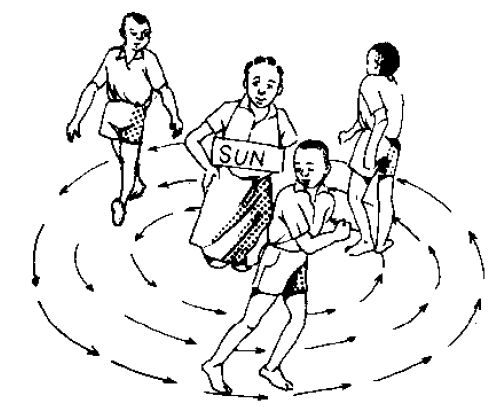
\includegraphics[width=0.4\textwidth]{./img/source/student-solar-system.png}
\end{center}

\begin{description*}
%\item[Subtopic:]{}
%\item[Materials:]{}
%\item[Setup:]{}
\item[Procedure:]{Place a chair at the centre of the football field of your school to represent the sun. Now ask 8 students to go around the chair in circles to represent the planets. The radius of each circle should correspond to the distance of the respective planet from the sun.

For examples, using a scale of 1 cm representing 1 million km from the sun, then the radius of Mercury must be 58 cm, that of Venus 107 cm, earth 149 cm, and so on. (Of course, in this scale, the sun would be a ball of 2 cm diameter, the earth only a grain of sand).}
%\item[Hazards:]{}
\item[Questions:]{What would the radii of the paths of Jupiter and Uranus be in this model?}
%\item[Observations:]{}
\item[Theory:]{They will be 7.8 m and 28.5 m respectively.
\begin{center}
\begin{tabular}{l r r}
\multicolumn{1}{l}{Planet} & \multicolumn{2}{p{0.2\textwidth}}{Distance in millions of km from sun}\\
&\\
Mercury & 58&\\
Venus & 107&\\
Earth & 149&\\
Mars & 227&\\
Jupiter & 773&\\
Saturn & 1418&\\
Uranus & 2853&\\
Neptune & 4469&
\end{tabular}
\end{center}}
%\item[Applications:]{}
\item[Notes:]{Pluto is no longer considered a planet, but revolves the sun at a radius of 5866 km.}
\end{description*}

\columnbreak

\subsection{Solar System Mobile}

%\begin{center}
%\includegraphics[width=0.4\textwidth]{./img/source/.png}
%\end{center}

\begin{description*}
%\item[Subtopic:]{}
\item[Materials:]{Flour, water, balloons, mixing bowl, strips of newspaper or old papers, string, sticks}
\item[Setup:]{Blow up nine balloons, one for each of the 8 planets and sun. Make a \nameref{sec:paper-mache} mixture with flour and water. Wet the paper strips in this mixture and apply to the balloons until you have a layer a couple papers-thick on each balloon. Leave each balloon slightly exposed at the bottom.}
\item[Procedure:]{When the papers are dried, pop the balloons inside. Use paint or marker pens to make the paper balls look like planets. Attach string and hang the planets in order around the sun.}
%\item[Hazards:]{}
%\item[Questions:]{Name the eight planets. Which planet is the largest? Smallest? Are they solid or gas?}
%\item[Observations:]{}
%\item[Theory:]{}
%\item[Applications:]{}
\item[Notes:]{Remember that the planets are all at different distance from the sun, but they are all in the same plane. For this reason, hang the planets at about the same height.}
\end{description*}

\subsection{Model of Sun-Earth-Moon}

\begin{center}
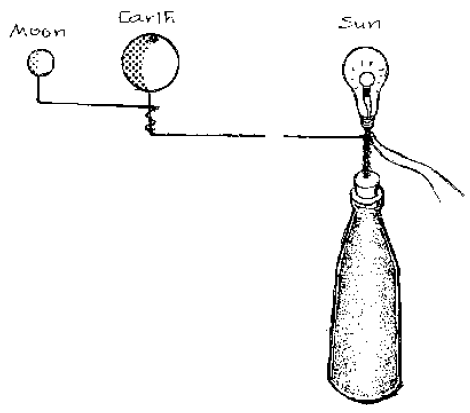
\includegraphics[width=0.4\textwidth]{./img/source/sun-earth-moon.png}
\end{center}

\begin{description*}
%\item[Subtopic:]{}
\item[Materials:]{Seed, fruit, bulb, stiff wires, bottle, sand}
%\item[Setup:]{}
\item[Procedure:]{Pierce a seed and a small fruit with wires. Join a bulb to a bottle filled with sand using a wire. Join the three wires so that they allow rotation.}
%\item[Hazards:]{}
%\item[Questions:]{}
\item[Observations:]{The seed, fruit and bulb represent the moon, earth and sun respectively. The bulb may be lit using a battery.}
\item[Theory:]{The model can be used to show the movement of the earth and moon around the sun and earth respectively. It can also show the eclipse of the moon and sun, when the earth shades the moon or the moon shades a part of the earth respectively.}
%\item[Applications:]{}
%\item[Notes:]{}
\end{description*}

%==================================================================================================%

\section*{Gravitational Force} \index{Forces! gravitational} \index{Gravity! force of}


\subsection{Centripetal Force}

\begin{center}
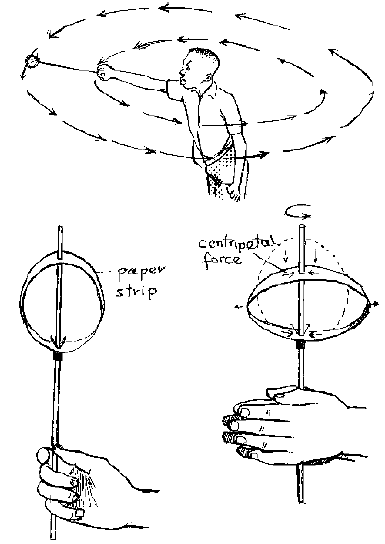
\includegraphics[width=0.4\textwidth]{./img/source/centripetal-force.png}
\end{center}

\begin{description*}
%\item[Subtopic:]{}
\item[Materials:]{Ball or stone, thread}
%\item[Setup:]{}
\item[Procedure:]{Tie a ball or sone to a thread and whirl it around as shown.}
%\item[Hazards:]{}
\item[Questions:]{What force keeps the stone on its circular track?}
%\item[Observations:]{}
\item[Theory:]{A force acts along the thread (which can be felt in your hand) called \emph{centripetal force} which keeps the stone in its circular path. A centripetal force also acts on each planet to keep it on its circular path.}
%\item[Applications:]{}
\item[Notes:]{Due to its inertia a body will move along a straight path when \emph{no} force acts on it. If the force of gravity between the planets and sun were suddenly turned off, they would drift out of their orbits in straight lines tangent to their orbits.}
\end{description*}

\columnbreak

\subsection{Bucket Swing}

\begin{center}
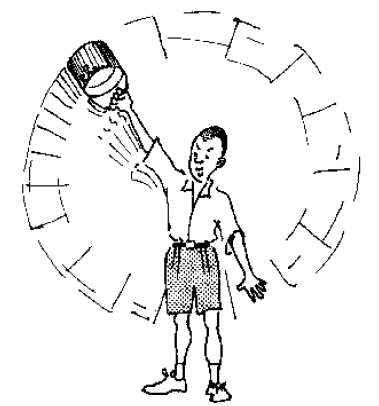
\includegraphics[width=0.4\textwidth]{./img/source/bucket-swing.png}
\end{center}

\begin{description*}
%\item[Subtopic:]{}
\item[Materials:]{Bucket, water, rope}
%\item[Setup:]{}
\item[Procedure:]{Swing a bucket partially filled with water in vertical circles over your head by holding a rope.}
%\item[Hazards:]{}
\item[Questions:]{What happens to the water inside?}
\item[Observations:]{When you swing the bucket with speed, the water remains in the bucket even when facing upside-down.}
\item[Theory:]{Centripetal force keeps the water forced against the bottom of the bucket, or away from the centre of its orbit. Similarly, there is a centripetal force between the planets and sun.}
%\item[Applications:]{}
%\item[Notes:]{}
\end{description*}

%==================================================================================================%

\section*{Constellations} \index{Constellations}


\subsection{Star Gazing}

%\begin{center}
%\includegraphics[width=0.4\textwidth]{./img/source/.png}
%\end{center}

\begin{description*}
%\item[Subtopic:]{}
%\item[Materials:]{}
%\item[Setup:]{}
\item[Procedure:]{Take the students out at night where there is little light from lamps and fires. Look for constellations, stars, planets and satellites. Discuss the reason for having constellations and the motion of the sky over the course of a night and a year.}
%\item[Hazards:]{}
%\item[Questions:]{}
\item[Observations:]{Especially in rural areas, the stars and other celestial bodies are very clear. Depending on the time of year, different planets and constellations will be visible. The most obvious constellations are Orion, Ursa Major and the Southern Cross. The brightest star is Sirius. If the sky is clear then our galaxy, the Milky Way, is visible as a bright stripe across the sky.}
%\item[Theory:]{}
%\item[Applications:]{}
%\item[Notes:]{}
\end{description*}

%==================================================================================================%

%\section*{The Earth and Its Moon}




%==================================================================================================%



\end{multicols}

\pagebreak